\documentclass[12pt, letterpaper]{article}
\usepackage[utf8]{inputenc}
\usepackage{amsmath}
\usepackage{graphicx}
\graphicspath{ {./slike/} }

\title{Seminarska naloga iz statistike}
\author{Žiga Gladek}

\renewcommand{\refname}{Literatura}

\begin{document}
\maketitle

\renewcommand{\abstractname}{Povzetek}
\begin{abstract}
V tem dokumentu so povzete obravnave nalog, ki sem jih preučeval v sklopu predmeta statistika na programu Matematika UN. Pri reševanju sem si pomagal s programskim jezikom Python, z orodjem Jupyter Notebook in s knjižnico pandas za branje datotek tipa csv. Za prikaze podatkov sem uporabljal knjižnico matplotlib. Za večino uporabljenih metod se sklicujem na zapiske iz predavanj, za preostanek pa na priporočeno literaturo~\cite{Rice}.
\end{abstract}

\section*{1. naloga: Kibergrad}

\subsubsection*{Točka a)} Najprej moramo vzeti enostavni slučajni vzorec $200$ družin in oceniti delež družin v Kibergradu, v katerih vodja gospodinjstva nima mature. To pomeni, da je v tabeli takega gospodinjstva stopnja izobrazbe $\leq 38$. Pravi delež bomo označili s $p$. Enostavni slučajni vzorec lahko v programu dobimo s pomočjo ukaza \emph{sample}. Nepristranska ocena za $p$ je:
\[
\hat{p} = \frac{\text{št. gospodinjstev v vzorcu brez mature}}{200}.
\]
Lahko si mislimo, da smo v enostavnem slučajnem vzorcu gospodinjstvom, v katerih ima vodja vsaj maturo, priredili število $0$, tistim, v katerih ima nižjo izobrazbo pa $1$. V tem primeru je ta ocena le povprečje vrednosti v dobljenem vzorcu. Če to implementiramo, nam program pove, da je $\hat{p} = 0,18500$. Seveda pri različnih vzorcih lahko dobimo drugačno oceno.

\subsubsection*{Točka b)} Ocenili bomo standardno napako, ki je po definiciji enaka $se = \sqrt{var(\hat{p})}$. Naj bo $N$ velikost populacije, $n$ velikost vzorca in $\sigma^2$ populacijska varianca. Potem vemo, da pri enostavnem slučajnem vzorcu velja formula
\[
se = \sqrt{\frac{N-n}{N-1}\frac{\sigma^2}{n}}.
\]
V resnici pa $\sigma^2$ še ne poznamo, zato moramo najprej oceniti še to. V našem primeru, kjer smo vse družine v vzorcu razdelili v dve skupini, velja $\sigma^2 = p(1-p)$. To znamo oceniti s pomočjo $\hat{p}$ kot $\hat{\sigma}^2 = \hat{p}(1 - \hat{p})$, vendar pa ta ocena ni nepristranska. Iz predavanj vemo, da jo lahko do nepristranske popravimo na naslednji način:
\[
\hat{\sigma}^2_+ = \frac{N-1}{N}\frac{n}{n-1} \hat{p}(1 - \hat{p}).
\]
S tem se lahko dokopljemo še do nepristranske ocene za standardno napako, tako da v formuli za standardno napako $\sigma^2$ zamenjamo s $\hat{\sigma}^2_+$. Dobimo:
\[
\hat{se}_+ = \sqrt{\frac{N-n}{N}\frac{1}{n-1}\hat{p}(1 - \hat{p})}.
\]
V našem primeru je $N = 43886$ in $n = 200$. Program nam sedaj pove, da je pri danem vzorcu $\hat{se}_+$ enaka približno $0,02746$. Na podlagi te ocene sedaj lahko izpeljemo še $95\%$ interval zaupanja za $p$. Da ga dobimo, bomo upoštevali, da je približno $\frac{\hat{p} - p}{\hat{se}_+} \sim Student(n-1)$. Pri stopnji tveganja $\alpha = 0,05$ dobimo aproksimativni interval zaupanja za $p$:
\[
p \in \left[\hat{p} - F_{Student(199)}^{-1}(0,975)\hat{se}_+, \quad \hat{p} + F_{Student(199)}^{-1}(0,975)\hat{se}_+\right].
\]
Ta je pri danih podatkih enak približno $[0,13062, 0,23938]$. Pri tem smo na podlagi tabele kvantilov Studentove porazdelitve upoštevali, da je $F_{Student(199)}^{-1}(0,975) \doteq 1,98$. Dejansko smo uporabili kvantil, ki ustreza $120$ prostostnim stopnjam, vendar je to za naše namene dovolj dober približek.

\subsubsection*{Točka c)} Poglejmo populacijski delež gospodinjstev, v katerih vodja gospodinjstva nima srednješolske izobrazbe. Ta delež je enak:
\[
p = \frac{\text{št. gospodinjstev brez mature}}{N} \doteq 0,21150.
\]
Naša točkovna ocena se od točne vrednosti torej razlikuje za slabe $3\%$, opazimo pa tudi, da prej dobljeni aproksimativni interval zaupanja pokrije populacijski delež.
S tem da poznamo $p$, lahko izračunamo tudi pravo standardno napako pri vzorcih velikosti $200$.
Upoštevajmo, da je $\sigma^2 = p(1-p)$. Tedaj je:
\[
se = \sqrt{\frac{N-n}{N-1}\frac{\sigma^2}{n}} = \sqrt{\frac{N-n}{N-1}\frac{p(1-p)}{n}} \doteq 0,02881.
\]
Približek $\hat{se}_+$ se torej od točne vrednosti razlikuje šele na tretji decimalki.

\subsubsection*{Točka d)} Vzeli bomo še $99$ enostavnih slučajnih vzorcev in za vsakega od teh določili $95\%$ interval zaupanja za $p$. S pomočjo programa dobimo, da je delež intervalov, ki pokrije populacijski delež enak $\frac{95}{100}$. Poglejmo si to še s sliko:
\begin{center}
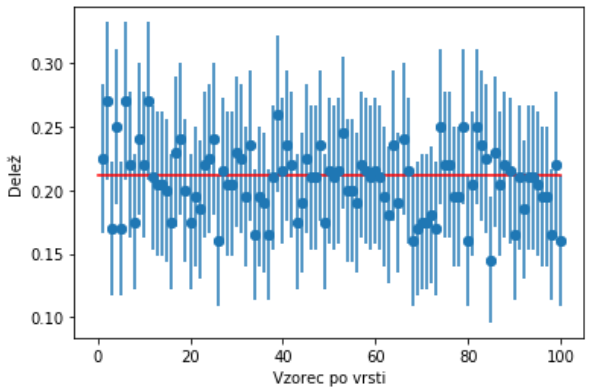
\includegraphics[scale=0.7]{Intervali}
\end{center}
Rdeča črta na sliki prikazuje populacijski delež, intervali zaupanja pa so narisani vertikalno, pri čemer je vrednost na sredini intervala dodatno označena z modro piko. Število intervalov, ki je pokrilo populacijski delež ni presenetljivo in kvečjemu potrdi, da smo pravilno določilli interval zaupanja, saj $95\%$ interval zaupanja pomeni ravno to, da bo populacijski delež v povprećju pokril v $95$ od $100$ primerih.

\subsubsection*{Točka e)} Izračunajmo standardne odklone vzorčnih deležev iz prejšnjih $100$ vzorcev in jih primerjajmo s pravo standardno napako pri vzorcih velikosti $200$, ki jo poznamo že od prej. Standardni odklon vzorčnega deleža $\hat{p}$ je enak $\sqrt{var(\hat{p})}$, kar pa je ravno standardna napaka. To vrednost lahko ocenimo na podlagi vsakega intervala posebej. Primerjavo teh s pravo vrednostjo nato lahko ponazorimo z grafikonom:
\begin{center}
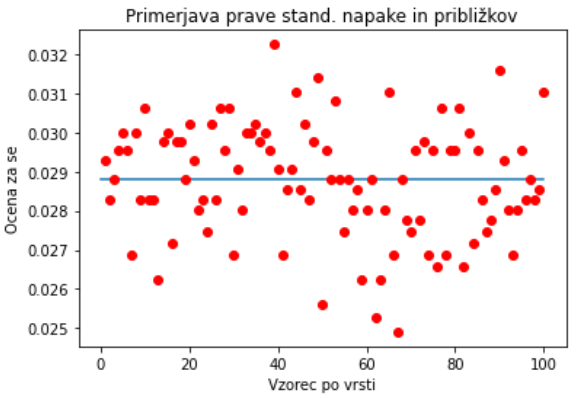
\includegraphics[scale=0.7]{SE_200_primerjava}
\end{center}
Pri tem modra vodoravna črta označuje pravo standardno napako pri vzorcih te velikosti.

\subsubsection*{Točka f)} Ponovimo prejšnji dve točki še za primer, ko so vzorci velikosti $800$, torej $n = 800$. Interval zaupanja za $p$ je tedaj oblike
\[
p \in \left[\hat{p} - F_{Student(799)}^{-1}(0,975)\hat{se}_+, \quad \hat{p} + F_{Student(799)}^{-1}(0,975)\hat{se}_+\right],
\]
pri čemer bomo vzeli $F_{Student(799)}^{-1}(0,975) = 1,97$. Seveda to ni točna vrednost, ampak bo za naše namene dovolj dober približek. Verjetno bi lahko tu vzeli tudi $1,98$ ali pa vrednost, ki je nekje vmes med tema dvema.
Delež intervalov, ki pokrije populacijski delež je znova enak $\frac{95}{100}$. Oglejmo si jih še s sliko:
\begin{center}
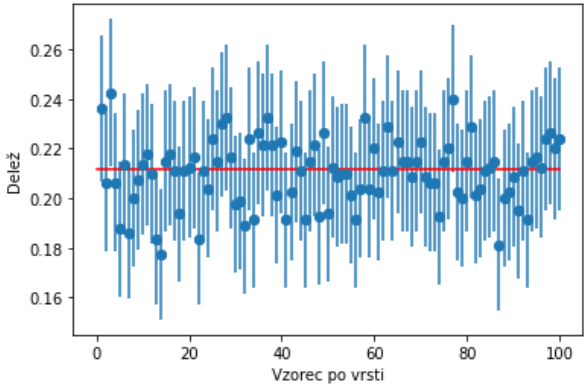
\includegraphics[scale=0.7]{Intervali_800}
\end{center}
Na prvi pogled ni vidnih razlik od prejšnjega primera, vendar pa so ti novi intervali dejansko ožji od tistih prej. Povprečna širina teh novih intervalov je enaka približno $0,05633$ v primerjavi s povprečjem v prejšnjem primeru, ki je bilo približno enako $0,11371$. Dejansko so intervali skoraj dvakrat ožji. Izkazalo se bo, da se to zgodi na račun približno dvakrat manjše standardne napake.

Populacijski delež seveda ni odvisen od vzorca in je enak kot prej. Za razliko od tega je prava standardna napaka pri vzorcu velikosti $800$ drugačna kot pri vzorcu velikosti $200$. Pri $n=800$ dobimo, da je $se \doteq 0,01431$, kar je občutno manj kot v prejšnjem primeru.
Poglejmo še, kako izgledajo približki za $se$, ki jih dobimo na podlagi dobljenih vzorcev.
\begin{center}
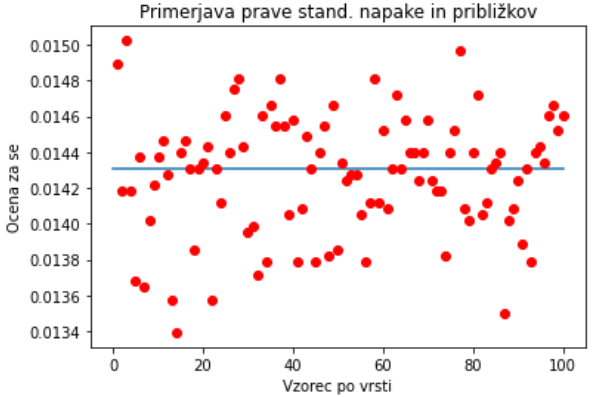
\includegraphics[scale=0.7]{SE_800_primerjava}
\end{center}
Sliki sicer izgledata podobno, vendar pa so približki v tem drugem primeru dejansko manj razpršeni okrog prave vrednosti, kot v prvem primeru, kar se vidi, če pogledamo vrednosti na $y$-osi. Da je standardna napaka v tem primeru manjša, ni presenetljivo, saj je le-ta merilo za to, kako natančno vzorčni delež aproksimira pravi delež. Že intuitivno je jasno, da če bo vzorec večji, bo natančnost boljša, se pa to vidi tudi iz eksplicitnega zapisa. Spomnimo se, da velja
\[
se = \sqrt{\frac{N-n}{N-1}\frac{\sigma^2}{n}}.
\]
Očitno je, da gre ta izraz proti $0$, ko gre $n$ proti $N$. Oglejmo si odvisnost $SE$ od velikosti vzorca za dani $N$ še z grafom.
\begin{center}
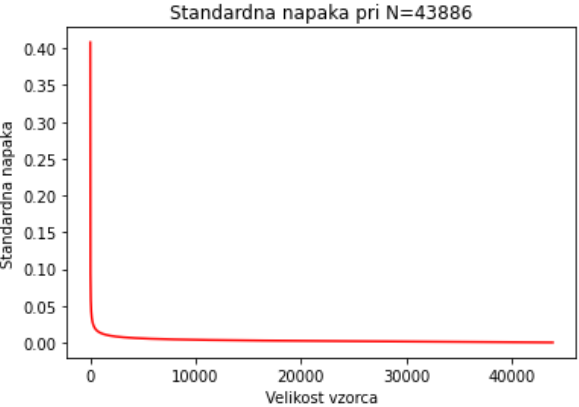
\includegraphics[scale=0.7]{stand_napaka_graf1}
\end{center}
Podrobeneje si lahko pogledamo, kako hitro pada pri vrednostih, s katerimi imamo opravka.
\begin{center}
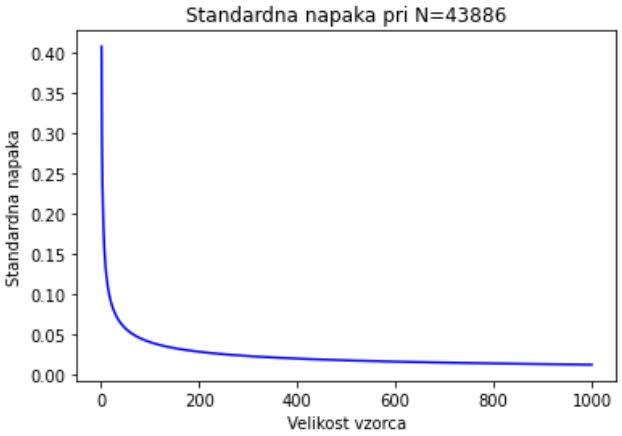
\includegraphics[scale=0.7]{stand_napaka_graf2}
\end{center}
Seveda je standardna napaka odvisna tudi od populacijske variance $\sigma^2$. Manjša kot je, manjše vzorce rabimo, da dobimo dobre približke. Opazimo pa še nekaj. Standardna napaka pri vzorcu velikosti $800$ je približno dvakrat manjša kot pri vzorcu velikosti $200$ in to ni naključje. Če zgornjo formulo zapišemo nekoliko drugače, dobimo
\[
se = \sqrt{1 - \frac{n-1}{N-1}}\frac{\sigma}{\sqrt{n}}.
\]
Če je $n$ majhen v primerjavi z $N$, je izraz pod korenom približno enak $1$, kar pomeni da je
\[
se \approx \frac{\sigma}{\sqrt{n}}.
\]
Iz tega izraza se vidi, da za dvakrat manjšo standardno napako, potrebujemo štirikrat večji vzorec, kar pa je ravno tisto, kar smo v našem primeru naredili. To razloži tudi razliko v širinah intervalov. Dolžina posameznega intervala je enaka $2\cdot1,98\cdot\hat{se}_+$. Ker je standardna napaka približno dvakrat manjša, se to odraža tudi v približkih $\hat{se}_+$, zato so intervali približno dvakrat ožji, kot v prvem primeru. Na kratko komentirajmo še kako je z rapršenostjo približkov za standardno napako okrog prave vrednosti. Omenili smo že, da je v drugem primeru ta razpršenost razvidno manjša. Da bi to kvantificirali, bi morali izračunati varianco približka $\hat{se}_+$. Ta je zaradi nepristranskosti, ravno enaka srednji kvadratični napaki te cenilke, kar pa vemo, da je v nekem smislu merilo za to, kako dobra je cenilka.
\[
MSE(\hat{se}_+) = var(\hat{se}_+) + Bias(\hat{se}_+)^2 = var(\hat{se}_+).
\]
Tega ne bomo popolnoma do konca izračunali, vendar se odvisnost od $n$ delno vidi že brez tega. Velja namreč:
\[
var(\hat{se}_+) = var\left(\frac{N-n}{N(n-1)}\hat{p}(1 - \hat{p})\right) = \left(\frac{N-n}{N(n-1)}\right)^2 var(\hat{p}(1 - \hat{p})).
\]
Seveda je $\hat{p}$ tudi odvisen od velikosti vzorca, vendar pa lahko še vedno dobimo približek, če izraz v oklepaju zapišemo drugače:
\[
\frac{N-n}{N}\frac{1}{n-1} = \left(1 - \frac{n}{N}\right)\frac{1}{n-1} \approx \frac{1}{n-1}.
\]
V zadnjem koraku smo upoštevali, da je v našem primeru $n$ majhen v primerjavi z $N$. Tako je
\[
var(\hat{se}_+) \approx \frac{1}{(n-1)^2}var(\hat{p}(1 - \hat{p}))
\]
Tu se že nekoliko vidi, kako bo razpršenost padala, ko vzorec povečujemo. Pričakujemo namreč, da bodo z večjimi vzorci boljši tudi približki za populacijsko varianco in da bo tudi razpršenost teh približkov padala.

\section*{2. naloga: TempPulz}

\begin{thebibliography}{99}
\bibitem{Rice} J. A.~Rice, \emph{Mathematical Statistics and Data Analysis, Third Edition}, Thomson Brooks/Cole, Duxbury, 2007
\end{thebibliography}

\end{document}

